\documentclass[letterpaper,11pt]{article}

\usepackage{amsmath}
\usepackage{amssymb}
\usepackage{booktabs}
\usepackage[hmargin=1.25in,vmargin=1in]{geometry}
\usepackage{graphicx}
\usepackage{hyperref}
\usepackage{listings}
\usepackage{lmodern}
\usepackage{mathtools}
\usepackage{microtype}
\usepackage{minted}

\DeclareMathOperator*{\argmin}{arg\,min}

\author{Philip Pham}
\date{\today}
\title{CSE 547 - Assignment 2}

\begin{document}
\maketitle

\section*{Problem 0}

\begin{description}
\item[List of collaborators:] I have not collaborated with anyone.
\item[List of acknowledgements:] None.
\item[Certify that you have read the instructions:] I have read and understood
  these policies.
\end{description}

\section*{Problem 1: Generalization, Streaming, and SGD}

In class, we examined using Stochastic Gradient Descent (SGD) for empirical loss
minimization, where we have an $N$ sized training set $\mathcal{T}$. The
empirical loss considered was:
\begin{equation}
  F(w) = \frac{1}{N} \sum_{(x,y) \in \mathcal{T}} l\left(w,(x,y)\right).
\end{equation}

Here, gradient descent for the function $F$ is the algorithm:
\begin{enumerate}
\item Initialize at some point $w^{(0)}$.
\item Sample $(x,y)$ uniformly at random from the set $\mathcal{T}$.
  \label{item:sgd_sample}
\item Update the parameters:
  \begin{equation}
    w^{(k+1)} = w^{(k)} - \eta_k \cdot \nabla l\left(w^{(k)},(x,y)\right),
  \end{equation}
  and go back to \ref{item:sgd_sample}.
\end{enumerate}

We provided guarantees assuming that $F$ was smooth and the gradients in our
training set were uniformly bounded,
$\lVert \nabla l\left(w, (x,y)\right) \rVert \leq B$.

However, in practice, we care about generalization, that is, statements on how
well we do on the underlying distribution. Define:
\begin{equation}
  \mathcal{L}(w) = \mathbb{E}_{(x,y) \in \mathcal{D}}l\left(w, (x,y)\right),
\end{equation}
where $\mathcal{D}$ is the underlying distribution.

Suppose we sought a point where $\lVert \nabla \mathcal{L} \rVert^2$ was
small. Obtaining this quantity to be small even in expectation would be
acceptable for this problem Assume that $\mathcal{L}$ is smooth and that the
gradients are uniformly bounded,
$\lVert \nabla l\left(w, (x,y)\right)\rVert \leq B$ for all parameters and all
possible points $(x,y)$ (under $\mathcal{D}$).

\begin{enumerate}
\item 
  Assume we have sampling access to our underlying distribution
  $\mathcal{D}$. Explain how we can make $\lVert \mathcal{L}(w) \rVert^2$ small
  in expection. What can you guarantee if you obtain $m$ samples and how would
  you do this?

  \subsection*{Solution}

  If we sample from $\mathcal{D}$ (as opposed to from $\mathcal{T}$ in Step
  \ref{item:sgd_sample} in the original algorithm), then we can guarantee that
  $\lVert \mathcal{L}(w) \rVert^2$ is small in expectation.

  

\item Suppose we contruct an $N$ sized training set $\mathcal{T}$, where each
  point is sampled under $\mathcal{D}$; then we construct the empirical loss
  funciton $F(w)$; then we run SGD on $F$ for $K$ steps (suppose $K \geq N$). Is
  there an argument on this procedure that implies something non-trivial (and
  technically correct) about $\lVert \nabla\mathcal{L}(w)\rVert^2$, even in
  expectation?

  \subsection*{Solution}
\end{enumerate}

\section*{Problem 2: GD versus Adaptive GD}

Let us compare gradient descent (GD), with a constant stepsize $\eta$, to
Adagrad on two simple one-dimensional objective functions. Adagrad will use the
stepsize at iteration $k$ where:
\begin{equation}
  \eta_k = \frac{C}{\sqrt{\sum_{j = 0}^k \lVert \nabla F \left(
        w^{(j)}
      \right)\rVert^2}}.
\end{equation}

\begin{enumerate}
\item Consider $F(w) = \frac{1}{2}w^2$. Let us start at $w_0 = 1$. For this
  problem a constant stepsize certainly makes sense for GD. Let $\eta = 3/4$ and
  $C = 3/4$.

  \begin{enumerate}
  \item Analytically, characterize the convergence rates of $GD$ and Adagrad
    with these parameter settings.

    \subsection*{Solution}
  \item Empircally, plot the learning curves, where the iteration is on the
    $x$-axis and the log of $F\left(w^{(k)}\right) - F_*$ on the $y$-axis.

    \subsection*{Solution}
  \end{enumerate}
  
\item Consider the non-smooth, convex function $F(w) = \lvert w \rvert$. Let us
  start with $w_0 = 1$. Use $\eta = 3/4$ and $C = 3/4$ as before.

  \begin{enumerate}
  \item Analytically, characterize the convergence rates of $GD$ and Adagrad
    with these parameter settings.

    \subsection*{Solution}
  \item Empircally, plot the learning curves, where the iteration is on the
    $x$-axis and the log of $F\left(w^{(k)}\right) - F_*$ on the $y$-axis.

    \subsection*{Solution}
  \end{enumerate}
\end{enumerate}

\section*{Problem 3: Understanding Non-Convexity}

\subsection*{Newton's Method}

The least squares problem can be written as:
\begin{equation}
  \min_{w}L(w),~\text{where}~L(w) \coloneqq \frac{1}{2N}\left\lVert Xw - Y\right\rVert^2,
\end{equation}
where $X$ is our $N \times d$ matrix and $Y$ is our $N \times 1$ output vector. If we define:
\begin{equation}
  \Sigma \coloneqq \frac{1}{N}X^\intercal X,~u = \frac{1}{N}X^\intercal Y,
\end{equation}
then, this expression can be written as
\begin{equation}
  L(w) = \frac{1}{2}w^\intercal\Sigma w - u^\intercal w + \frac{1}{2N}\lVert Y \rVert^2.
\end{equation}

Note that $\Sigma$ is a positive-definite matrix. Assume that $\Sigma$ is full
rank.

Newton's method is typically thought of a being better than gradient descent due
to it using second order information. At some $w_0$, the method first constructs
a second-order Taylor's approximation around $w_0$, and then it makes the new
iterate to be the point at which the gradient of this approximation is $0$, that
is,
\begin{equation}
  w \leftarrow w - \left[ \nabla^2 L(w) \right]^{-1} \nabla L(w).
  \label{eqn:newton_update}
\end{equation}

\begin{enumerate}
\item Starting at some $w_0$ write out one step of the Newton's method in terms
  of $\Sigma$ and $u$. If you take one step, what point do you get to?

  \subsubsection*{Solution}

  Since $\Sigma$ is positive-definite, we can write $\Sigma = PD^2P^\intercal$,
  where $D$ is diagonal. Using that
  $w^\intercal \Sigma w = \left(D P^\intercal
    w\right)^\intercal\left(DP^\intercal w\right)$ and the chain rule, we have
  that
  \begin{align}
    \nabla L(w)
    &= D\left(L(w)\right)^\intercal \nonumber\\
    &= \left(\frac{1}{2} \left(2w^\intercal PD\right)\left(D P^\intercal\right)  - u^\intercal\right)^\intercal \nonumber\\
    &= \left(w^\intercal \Sigma - u^\intercal\right)^\intercal \nonumber\\
    &= \Sigma w - u.
      \label{eqn:newton_grad}
  \end{align}

  Calculating the derivative again, we have obtain
  \begin{equation}
    \nabla^2 L\left( w \right) = \Sigma.
    \label{eqn:newton_hessian}
  \end{equation}

  Subtituting Equations \ref{eqn:newton_grad} and \ref{eqn:newton_hessian} into
  Equation \ref{eqn:newton_update}, we obtain
  \begin{equation}
    w_1 = w_0 - \Sigma^{-1}\left(
      \Sigma w_0 - u
    \right) = \boxed{\Sigma^{-1} u.}
    \label{eqn:newton_w1}
  \end{equation}
  
\item Comment on the loss of this point and how it compares to the minimal
  function value?
  
  \subsubsection*{Solution}

  Equation \ref{eqn:newton_w1} expands to
  \begin{equation}
    w_1 = \Sigma^{-1} u = \left(X^\intercal X\right)^{-1}X^\intercal Y,
  \end{equation}
  which is the solution to the least squares problem, so $L(w_1)$ is the global
  minimum function value.
\end{enumerate}

\subsection*{Non-convex Case}

Consider the objective function:
\begin{equation}
  F(w) = \frac{1}{2}w^\intercal A w - b^\intercal w + c,
\end{equation}
where $A$ is a symmetric matrix, $b$ is a vector, and $c$ is a scalar. Our goal
is to minimize the objective function. Assume that $\Sigma$ is full rank.

Assume that $A$ is still symmetric, yet suppose now that there is at least one
negative eigenvalue. Hence, the problem is non-convex. Again, suppose you start
at $w_0$ and take a step of Newton's method. Let this new point be $w_1$.

\begin{enumerate}
\item What is the point $w_1$ and the object value $F\left(w_1\right)$.

  \subsubsection*{Solution}

  The calcuation for the gradient is similar to that in Equation
  \ref{eqn:newton_grad}:
  \begin{equation}
    \nabla F(w) = Aw - b.
    \label{eqn:newton_grad2}
  \end{equation}
  It's notable that $D$ will now have at least one complex entry on its
  diagonal. However, we only $D$ for an intermediate step. The final solution
  will still contain real values.

  Then, the Hessian is constant-valued:
  \begin{equation}
    \nabla^2 F(w) = A.
    \label{eqn:newton_hessian2}
  \end{equation}

  Substituting Equations \ref{eqn:newton_grad2} and \ref{eqn:newton_hessian2}
  into Equation \ref{eqn:newton_update}, we get that
  \begin{equation}
    w_1 = w_0 - A^{-1}\left(Aw_0 - b\right) = \boxed{A^{-1}b.}
    \label{eqn:newtwon_w12}
  \end{equation}
  The objective value is
  \begin{align}
    F\left(w_1\right)
    &= \frac{1}{2} \left(b^\intercal A^{-1}\right)A\left(A^{-1}b\right)
      - b^\intercal \left(A^{-1}b\right) + c \nonumber\\
    &= \boxed{-\frac{1}{2}b^\intercal A^{-1}b + c.}
      \label{eqn:newton_min_object2}
  \end{align}
  
\item What is the gradient at $w_1$?
  \subsubsection*{Solution}

  Substituting Equation \ref{eqn:newtwon_w12} into Equation
  \ref{eqn:newton_grad}, we get that
  \begin{equation}
    \nabla F(w_1) = Aw_1 - b = \boxed{0.}
  \end{equation}  
\item What is the minimal object value of $F\left(\cdot\right)$? Did we achieve
  it?

  \subsubsection*{Solution}

  The minimal objective value is $-\infty$. We did not achieve it, for Equation
  \ref{eqn:newton_min_object2} is finite.

  To see that the minimal objective value is $-\infty$. Let $v$ be an
  eigenvector of $A$ associated with eigenvalue $\lambda < 0$. Then, we have
  \begin{align*}
    F\left(v\right)
    &= \frac{1}{2}v^\intercal A v - b^\intercal v + c \\
    &= \frac{\lambda}{2}\lVert v \rVert^2 - b^\intercal v + c.
  \end{align*}
  $\left\lvert b^\intercal v \right\rvert \leq \lVert b \rVert \lVert v \rVert$,
  so by increasing the magnitude of $v$, we can push the function value towards
  infinity.
\item Suppose you now are at $w_1$. In terms of the eigendecomposition
  $A = UDU^\intercal$, what are the directions of movement which \emph{strictly}
  decrease the objective value from $w_1$? Why?

  \subsubsection*{Solution}

  Let $v$ be an eigenvector with a negative eigenvalue. Then, for any
  $\epsilon > 0$, we have that
  \begin{equation*}
    \nabla F(w_1 + \epsilon v) = A\left(w_1 + \epsilon v\right) - b = \epsilon\lambda v,
  \end{equation*}
  where $\lambda < 0$ is the eigenvalue associated with $v$.
  
  By definition,
  $D_vF(w_1 + \epsilon v) = \nabla F(w_1 + \epsilon v) \cdot v = \epsilon\lambda
  \lVert v\rVert^2 < 0$, so $F$ is always decreasing in the direction $v$
  relative to $w_1$. This will be true for any $v$ that is a linear combination
  of eigenvectors with negative eigenvalues.
\end{enumerate}

\section*{Problem 4: Empirical Optimization}

We will now consider the multi-label classification problem. In the multi-label
problem, there are multiple labels that could be ``on'' for each input $x$. You
will use either the square loss or the binary logistic loss and consider
training two models, namely (i) a linear model and (ii) a multi-layer perceptron
(MLP) with a number of hidden nodes that you will tune.

You will try out three methods in each of the following: (1) SGD with a
mini-batch size that you tune. You will use the same minibatch size for the
other algorithms; (2) try out Polyak’s ``heavy ball method'' (aka momentum) or
Nesterov’s accelerated gradient descent (NAG); and (3) either Adagrad or
Adam. You must tune all the parameters of these methods.

The dataset contains 18 total categories with a number of categories for each
supercategory (vehicle or animal). In the dataset provided, each image contains
objects of a single supercategory, say vehicle, and potentially multiple objects
from the supercategory, such as car, boat, etc. In this exercise we shall build
a classifier that learns to identify \emph{all the categories of objects}
present in each image, by optimizing either a square loss or a logistic loss
objective. For the purposes of learning these classifiers, we shall use the
dataset and features from the first homework. We shall also provide a larger
version of this dataset since we need to train more parameters for this model.

The object function we choos to optimize is
\begin{equation}
  L(w) = \frac{\lambda}{2}\lVert w \rVert^2 +
  \frac{1}{n}\sum_{i=1}^n\sum_{j=1}^k l\left(y_{ij},f_{ij}(w)\right),  
\end{equation}
where $f_{ij}(w) = w_j^\intercal x_i$ and $w_j \in \mathbb{R}^d$ is the $j$th
column of $w \in \mathbb{R}^d \times \mathbb{R}^k$. Here, $w$ is the linear
model we wish to optimize over and $\lambda > 0$ is the strength of $l_2$
regularization. here $l$ is the loss function:
\begin{itemize}
\item $l\left(y,\hat{y}\right) = \frac{1}{2}\left(y - \hat{y}\right)^2$ is the square error
  loss.
\item
  $l\left(y,\hat{y}\right) = y\log\left(1 + \exp\left(-\hat{y}\right)\right) +
  (1-y)\log\left(1 + \exp\left(\hat{y}\right)\right)$ is the logistic loss where
  the true label $y \in \{0,1\}$.
\end{itemize}

Notice that we encode $y_i$ as binary vector of length $k = 18$ (the number of
categories) where a $1$ indicates the presence of a category and $0$ indicates
the absence.

Determine which loss function works better for a linear classifier and use that
loss throughout the question.

When using $MLP$,
$f_{ij}(w) = \left\langle w_j^{(2)},
  \operatorname{relu}\left(w^{(1)}x_i\right)\right\rangle$, where
$w^{(1)} \in \mathbb{R}^h \times \mathbb{R}^d$ are the weights in the first
layer and $h$ is the number of hidden nodes. Again $w_j^{(2)} \in \mathbb{R}^h$
is the $j$th column of $w^{(2)} \in \mathbb{R}^h \times \mathbb{R}^k$, the
weights of the second layer.

\subsection*{SGD and Linear Regression}

Now consider running stochastic gradient descent on $L(w)$.

\begin{enumerate}  
\item What mini-batch size do you use? What stepsize did you use? What value of
  $\lambda$ did you use? Specify your stepsize scheme if you chose to decay your
  stepsize. Which loss function did you find works better?

  \subsubsection*{Solution}

  I used a mini-batch size of $8$. My learning rate was $10^{-4}$. I used
  $\lambda = 0.7$. I found logistic loss to work better.
  
\item Report your training and validation loss.

  \subsubsection*{Solution}

  The results for the linear model can be seen in Figure
  \ref{fig:linear_loss_sgd} and Table \ref{tab:linear_sgd}. Training loss was
  0.122861 and validation loss was 0.199776.
  
  \begin{figure}
    \centering
    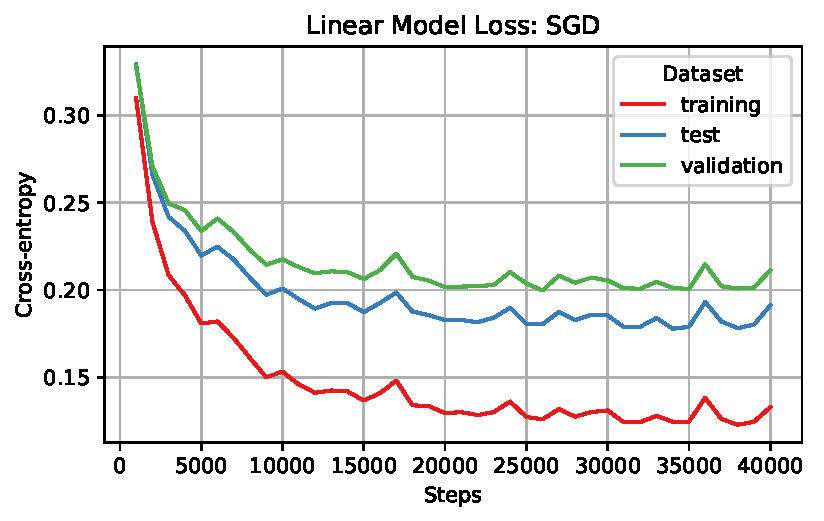
\includegraphics{problem4/linear_loss_sgd.pdf}
    \caption{Some overfiiting likely occurred since training loss is
      significantly less that validation loss. Increasing $\lambda$ made the
      model perform worse, however.}
    \label{fig:linear_loss_sgd}
  \end{figure}

  \begin{table}
    \centering
    \begin{tabular}{lrr}
      \toprule
      {} &  Average Precision Score &      Loss \\
      \midrule
      Training   &                 0.871461 &  0.122861 \\
      Validation &                 0.563140 &  0.199776 \\
      Test       &                 0.636070 &  0.177882 \\
      \bottomrule
    \end{tabular}
    \caption{Best average precision score and loss when training the linear
      model with SGD.}
    \label{tab:linear_sgd}
  \end{table}

  The results for the MLP model can be seen in Figure \ref{fig:mlp_loss_sgd} and
  Table \ref{tab:mlp_sgd}. Training loss was 0.157085 and validation loss was
  0.190817. I used $\lambda = 0.05$ as my regularization parameter and 1 layer
  of 256 hidden units. The learning rate was 0.0005. Validation loss is better
  than the linear model, but test loss is worst.

  \begin{figure}
    \centering
    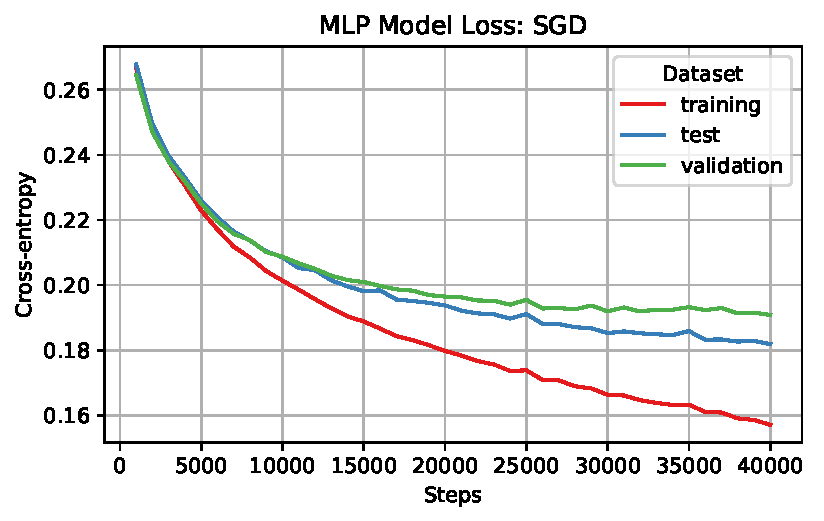
\includegraphics{problem4/mlp_loss_sgd.pdf}
    \caption{The model appears to not have converged yet.}
    \label{fig:mlp_loss_sgd}
  \end{figure}

  \begin{table}
    \centering
    \begin{tabular}{lrr}
      \toprule
      {} &  Average Precision Score &      Loss \\
      \midrule
      Training   &                 0.708156 &  0.157085 \\
      Validation &                 0.565152 &  0.190817 \\
      Test       &                 0.596515 &  0.181875 \\
      \bottomrule
    \end{tabular}
    \caption{Best average precision score and loss when training the MLP
      model with SGD.}
    \label{tab:mlp_sgd}
  \end{table}
  
\item Compute the average precision score in the same manner, and plot these
  quantities.

  \subsubsection*{Solution}

  The results are in Tables \ref{tab:linear_sgd} and \ref{tab:mlp_sgd}. See
  Figures \ref{fig:linear_average_precision_score_sgd} and
  \ref{fig:mlp_average_precision_score_sgd}
  
  \begin{figure}
    \centering
    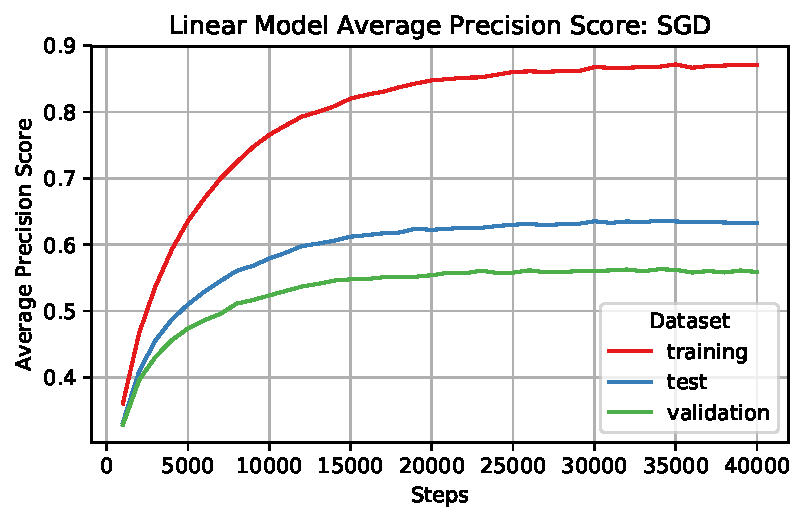
\includegraphics{problem4/linear_average_precision_score_sgd.pdf}
    \caption{Average precision score by the number of steps for the linear
      model.}
    \label{fig:linear_average_precision_score_sgd}
  \end{figure}
  
  \begin{figure}
    \centering
    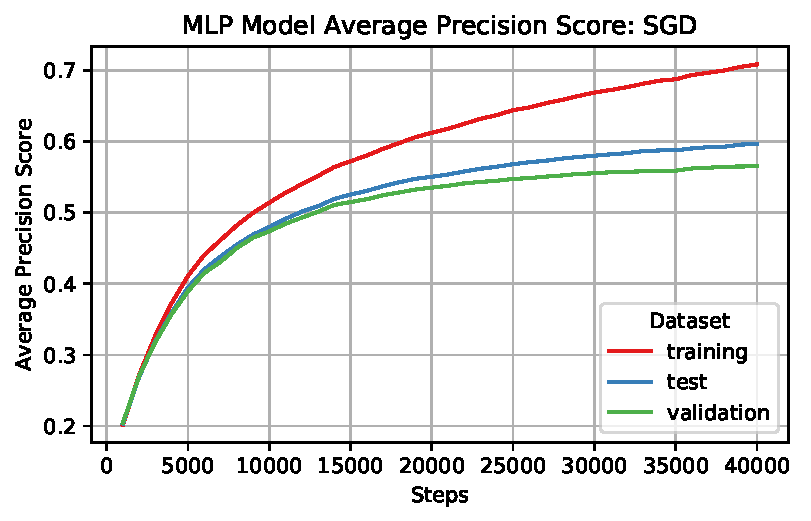
\includegraphics{problem4/mlp_average_precision_score_sgd.pdf}
    \caption{Average precision score by the number of steps for the multi-layer
      perceptron model.}
    \label{fig:mlp_average_precision_score_sgd}
  \end{figure}

\item Report the overall average precision score on the test set. Also report
  the average precision score for each of the 18 classes separately. Comment on
  how the AP scores relate to the class imbalance.

  \subsubsection*{Solution}

  Sorry, I ran out of time and didn't get this far :(.
  
\end{enumerate}

\subsection*{Nesterov's method}

I used Nesterov's method with a momentum parameter of 0.9. All other parameter
were the same as last section. The results can be seen in Tables
\ref{tab:linear_nesterov} and \ref{tab:mlp_nesterov}. The precision for the MLP
model is notably better with an average precision score of 0.629526 on the test
set.

The progress of the training runs can be seen in Figures
\ref{fig:linear_loss_nesterov}, \ref{fig:mlp_loss_nesterov},
\ref{fig:linear_average_precision_score_nesterov}, and
\ref{fig:mlp_average_precision_score_nesterov}.

  \begin{table}
    \centering
    \begin{tabular}{lrr}
      \toprule
      {} &  Average Precision Score &      Loss \\
      \midrule
      Training   &                 0.759774 &  0.170063 \\
      Validation &                 0.521453 &  0.262688 \\
      Test       &                 0.581486 &  0.232664 \\
      \bottomrule
    \end{tabular}
    \caption{Best average precision score and loss when training the linear
      model with SGD and Nesterov's momentum.}
    \label{tab:linear_nesterov}
  \end{table}

    \begin{table}
      \centering
      \begin{tabular}{lrr}
        \toprule
        {} &  Average Precision Score &      Loss \\
        \midrule
        Training   &                 0.793293 &  0.141046 \\
        Validation &                 0.587959 &  0.188455 \\
        Test       &                 0.629526 &  0.177171 \\
        \bottomrule
      \end{tabular}
      \caption{Best average precision score and loss when training the MLP
        model with SGD and Nesterov's momentum.}
    \label{tab:mlp_nesterov}
  \end{table}


  \begin{figure}
    \centering
    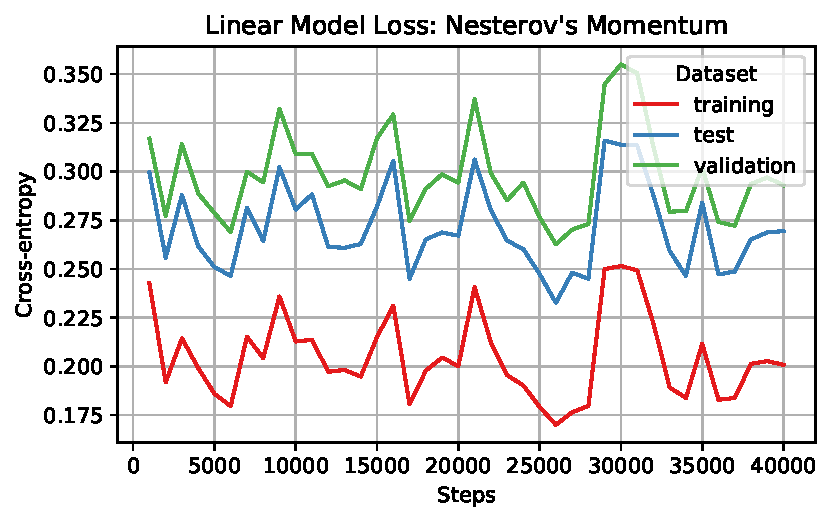
\includegraphics{problem4/linear_loss_nesterov.pdf}
    \caption{Evaluations on the datasets while training the linear model with
      Nesterov's momentum.}
    \label{fig:linear_loss_nesterov}
  \end{figure}

    \begin{figure}
    \centering
    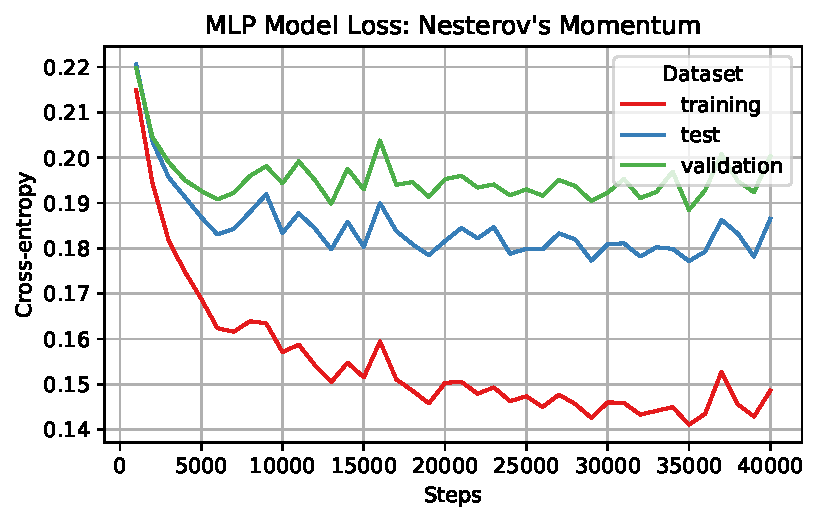
\includegraphics{problem4/mlp_loss_nesterov.pdf}
    \caption{Evaluations on the datasets while training the MLP model with
      Nesterov's momentum.}
    \label{fig:mlp_loss_nesterov}
  \end{figure}

  \begin{figure}
    \centering
    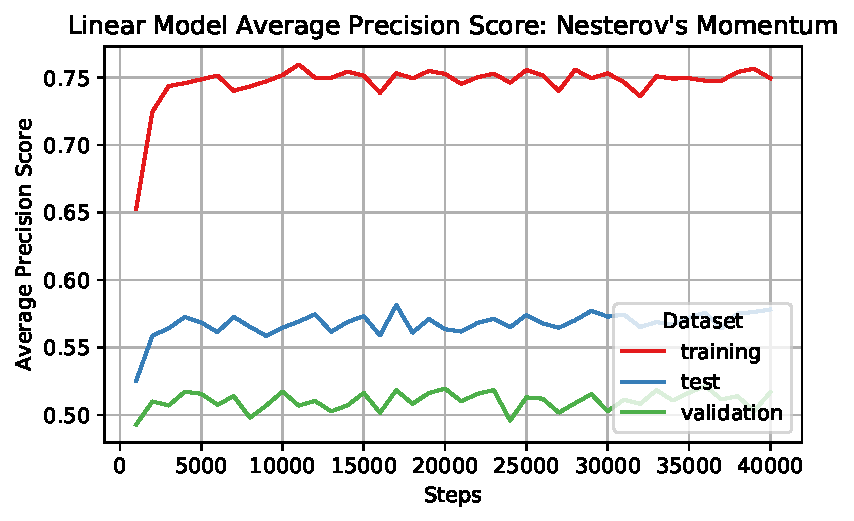
\includegraphics{problem4/linear_average_precision_score_nesterov.pdf}
    \caption{Average precision score by the number of steps for the linear
      model.}
    \label{fig:linear_average_precision_score_nesterov}
  \end{figure}
  
  \begin{figure}
    \centering
    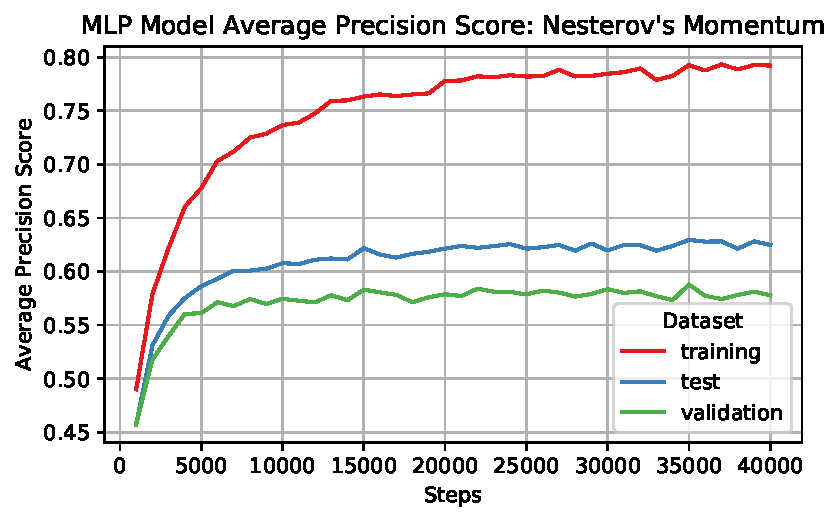
\includegraphics{problem4/mlp_average_precision_score_nesterov.pdf}
    \caption{Average precision score by the number of steps for the multi-layer
      perceptron model.}
    \label{fig:mlp_average_precision_score_nesterov}
  \end{figure}

\subsection*{Adagrad}

\end{document}
% Local Variables:
% TeX-command-extra-options: "-shell-escape"
% End: